% !TeX program = pdflatex
% Standalone source. Compile with pdfLaTeX; no external figures are required.
\documentclass[11pt,a4paper]{article}
\usepackage[margin=20mm]{geometry}
\usepackage[T1]{fontenc}
\usepackage{lmodern}
\usepackage{amsmath,amssymb,booktabs,array,xcolor,tikz,fancyhdr,hyperref,listings,pgfplots}
\usetikzlibrary{calc,arrows.meta}
\hypersetup{colorlinks=true,linkcolor=blue!50!black,urlcolor=blue!50!black}
\definecolor{accent}{HTML}{124E66}
\definecolor{pcol}{HTML}{A24021}
\definecolor{ncol}{HTML}{175A86}
\pagestyle{fancy}\fancyhf{}\fancyhead[L]{\small EE3032 / Fall 2016 / HW3}
\fancyhead[R]{\small CMOS logic}\fancyfoot[C]{\thepage}
\setlength{\headheight}{15pt}\setlength{\parindent}{0pt}\setlength{\parskip}{6pt}
\renewcommand{\arraystretch}{1.2}
\newcommand{\answer}[1]{\par\noindent\colorbox{accent!9}{\parbox{0.96\linewidth}{#1}}\par}
\newcommand{\AND}{\,}
\newcommand{\VDD}{V_{\mathrm{DD}}}
\newcommand{\VSS}{V_{\mathrm{SS}}}
% A conventional switch-level MOS symbol: continuous channel, insulated gate,
% and a gate bubble for pMOS. Bulk terminals are omitted, as explained below.
% Arguments: device id, x, y, gate literal, p or n. t/b are upper/lower terminals.
\newcommand{\MOS}[5]{
  \coordinate (#1) at (#2,#3);
  \coordinate (#1t) at ($(#1)+(0,.55)$);
  \coordinate (#1b) at ($(#1)+(0,-.55)$);
  \draw (#1t)--($(#1)+(0,.30)$)--($(#1)+(-.18,.30)$);
  \draw ($(#1)+(-.18,.34)$)--($(#1)+(-.18,-.34)$);
  \draw ($(#1)+(-.18,-.30)$)--($(#1)+(0,-.30)$)--(#1b);
  \draw ($(#1)+(-.35,.33)$)--($(#1)+(-.35,-.33)$);
  \def\type{#5}\def\ptype{p}
  \ifx\type\ptype
    \draw ($(#1)+(-.78,0)$)--($(#1)+(-.53,0)$);
    \draw ($(#1)+(-.465,0)$) circle (.065);
    \draw ($(#1)+(-.40,0)$)--($(#1)+(-.35,0)$);
  \else
    \draw ($(#1)+(-.78,0)$)--($(#1)+(-.35,0)$);
  \fi
  \node[anchor=east] at ($(#1)+(-.82,0)$) {$#4$};
  \node[anchor=west,font=\scriptsize] at ($(#1)+(.10,0)$) {#1};
}
% A transmission-gate instance; its two MOS devices are expanded on page 3.
\newcommand{\TG}[4]{
  \node[draw,rounded corners=1pt,minimum width=11mm,minimum height=6mm,
        fill=accent!5,font=\small] (#1) at (#2,#3) {$\mathrm{TG}_{#4}$};
}

\pgfplotsset{compat=1.18}
\lstset{basicstyle=\ttfamily\scriptsize,breaklines=true,frame=single,columns=fullflexible}
\begin{document}
\begin{center}{\LARGE\bfseries 2016 HW3}\\[4pt]{\large Equal-size AND Gate and Short-circuit Power}\\[4pt]{\small EE3032 / Introduction to VLSI Design}\end{center}
The original prompt and all supplied completed answers were read first. Both questions are independently solved and verified with actual local CIC018 TT HSPICE simulations. Sources, hashes, and corrections are in the year source ledger.
\textbf{Coverage.} HW3 is independently specified. No original HW1, HW2, or HW4 prompt was supplied for 2016; those assignments are not reconstructed from student answers.

\section*{1. Equal-size six-transistor AND gate}
The internal node is $F=\overline{AB}$, and the final output is $Z=AB$. \textbf{All six transistors have the same size}, as required:
\[
 \boxed{W=0.60\,\mu\mathrm m,\quad L=0.18\,\mu\mathrm m\quad\text{for every pMOS and nMOS}.}
\]
\begin{center}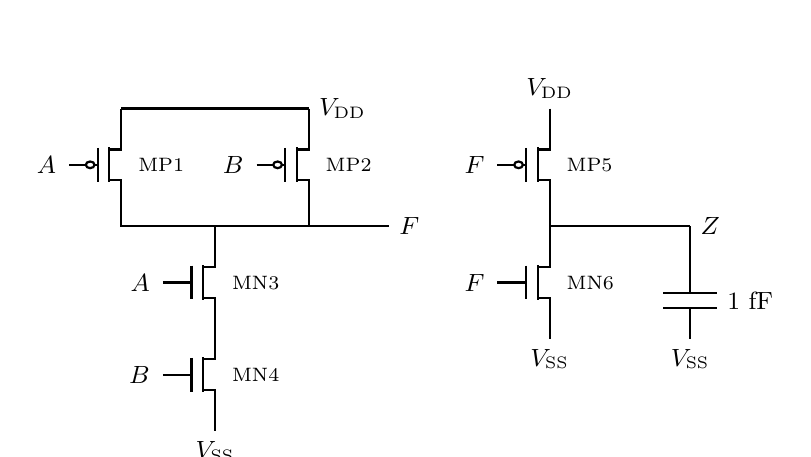
\begin{tikzpicture}[x=.85cm,y=.65cm,line width=.8pt,font=\small]
\MOS{MP1}{0}{6}{A}{p}\MOS{MP2}{2.8}{6}{B}{p}
\MOS{MN3}{1.4}{3.7}{A}{n}\MOS{MN4}{1.4}{1.9}{B}{n}
\draw (0,7.1)--(2.8,7.1) node[right] {$\VDD$};\draw (0,7.1)--(MP1t) (2.8,7.1)--(MP2t);
\draw (MP1b)--(0,4.8)--(4,4.8) node[right] {$F$};\draw (MP2b)--(2.8,4.8);
\draw (1.4,4.8)--(MN3t) (MN3b)--(MN4t);\draw (MN4b)--(1.4,.8) node[below] {$\VSS$};
\MOS{MP5}{6.4}{6}{F}{p}\MOS{MN6}{6.4}{3.7}{F}{n}
\draw (6.4,7.1) node[above] {$\VDD$}--(MP5t);
\draw (MP5b)--(MN6t);\draw (6.4,4.8)--(8.5,4.8) node[right] {$Z$};\draw (MN6b)--(6.4,2.6) node[below] {$\VSS$};
\draw (8.5,4.8)--(8.5,3.5);\draw (8.1,3.5)--(8.9,3.5) (8.1,3.2)--(8.9,3.2);\draw (8.5,3.2)--(8.5,2.6) node[below] {$\VSS$};\node[right] at (8.9,3.35) {1 fF};
\end{tikzpicture}\end{center}
Every pMOS bulk connects to VDD and every nMOS bulk to VSS. The testbench declares a 1 fF Z load, because the prompt leaves the load unspecified; the inverter gate provides the natural F load. Conditions are TT, $25^\circ$C, 1.8 V supply, 100 ps input rise/fall time, and \texttt{DELMAX=2p}. This nominal supply and declared load make the simulation fully reproducible; other choices change the delay numbers.
The three bidirectional families 00$\leftrightarrow$11, 01$\leftrightarrow$11, and 10$\leftrightarrow$11 cover all primary-input transitions that change the ideal outputs. Each family is simulated over three cycles. Delays use input and output 50\% crossings (0.9 V), with the changing input as the trigger; A/B coincide in the 00 case.
\begin{center}\begin{tabular}{lrrrr}\toprule
First-cycle case&$F_{HL}$&$F_{LH}$&$Z_{HL}$&$Z_{LH}$\\
&ps&ps&ps&ps\\\midrule
00$\to$11$\to$00&43.599&37.745&53.720&76.753\\
01$\to$11$\to$01&33.262&55.095&72.318&66.828\\
10$\to$11$\to$10&38.667&70.241&87.606&72.111\\
\bottomrule\end{tabular}\end{center}
\newpage
Taking the maxima of all 36 actual measurements gives:
\begin{center}\begin{tabular}{lcrcc}\toprule
Node&Direction&Worst delay (ps)&Initial AB&Cycle\\\midrule
F&HL&43.599&00&1\\
F&LH&70.256&10&3\\
Z&HL&87.606&10&1\\
Z&LH&76.753&00&1\\
\bottomrule\end{tabular}\end{center}
All four truth-table states are checked with six samples: initial states at 4 ns and the 11 state at 9 ns. Every low is below 0.2 V and every high exceeds 1.6 V. The largest F falling delay occurs when both inputs rise into 11; the largest F rising/Z falling delays occur in 11$\to$10, when the upper on-device also charges the stack node.
\textbf{Reference comparison.} One supplied answer uses equal 0.5$\,\mu$m widths and a very long input slew; another uses equal 0.36$\,\mu$m widths and 1 ps edges. Their delays differ accordingly. The latter ties the upper stacked nMOS bulk to its moving source node; we use the standard shared p-substrate/VSS bulk tie. We retain the useful equal-size circuit and transition table, include all six directed transitions, and report F/Z polarities separately. One reference's transition labels are inconsistent, so its printed worst-case statement is not copied.

\section*{2. Correct cycle-average short-circuit power}
Use an inverter with $W_p=1.44\,\mu$m, $W_n=0.36\,\mu$m, and $L=0.18\,\mu$m, at 1.8 V and TT/25$^\circ$C. The input has 3 ns rising/falling ramps,40 ns high pulse width, and 86 ns period. Sweep
\[
 C_L=0.1,0.3,0.5,0.7,1.0\ \mathrm{pF}.
\]
The prompt prints ``0.5pdf once; the surrounding list and reference materials identify this as 0.5 pF. The 3 ns edge durations are shown explicitly in the original figure.

Short-circuit power is simultaneous channel conduction through both devices, not the energy stored in $C_L$ and not the maximum of a power pulse. HSPICE's intrinsic channel-current probe \texttt{LX4(MOS)} has positive normal-conduction magnitudes for both the stated nMOS and pMOS orientations. Define
\[
 I_{sc}(t)=\max\{0,\min[I_{p,\mathrm{ch}}(t),I_{n,\mathrm{ch}}(t)]\},
 \quad P_{sc}=\frac{\VDD}{T}\int_{t_0}^{t_0+T}I_{sc}(t)\,dt.
\]
When the output falls, the pMOS channel current is the overlap component; when it rises, the nMOS channel current is the overlap component. Taking the smaller channel current removes the additional charging/discharging current supplied by the capacitor. Using intrinsic channel IDS excludes MOS displacement-current spikes. Off-state direct-path leakage remains in this operational integral but is negligible at the displayed precision.
The second full period 91--177 ns is integrated after startup. Both edge widths and the full 86 ns cycle are therefore accounted for. The following definitions are executed by HSPICE:
\begin{lstlisting}
.measure tran isc AVG PAR('max(0,min(lx4(mp),lx4(mn)))')
+ from=91n to=177n
.measure tran psc PARAM='1.8*isc'
.measure tran elsc PARAM='psc*86n'
.measure tran ptotal AVG PAR('-1.8*i(vvdd)')
+ from=91n to=177n
\end{lstlisting}
\newpage
\begin{center}\begin{tabular}{rrrrr}\toprule
$C_L$ (pF)&$P_{sc}$ ($\mu$W)&$E_{sc}$ (fJ)&$P_{load}$ ($\mu$W)&$P_{supply}$ ($\mu$W)\\\midrule
0.1&0.786014&67.597&3.767&4.685\\
0.3&0.442160&38.026&11.302&11.882\\
0.5&0.313114&26.928&18.837&19.291\\
0.7&0.243484&20.940&26.372&26.758\\
1.0&0.183094&15.746&37.674&38.001\\
\bottomrule\end{tabular}\end{center}
$P_{load}=C_L\VDD^2/T$ is the explicit load's ideal switching contribution. $P_{supply}$ is independently measured from the supply source; it includes short circuit, explicit-load switching, intrinsic-capacitance switching, and leakage. It is not equal to $P_{sc}$.
\begin{center}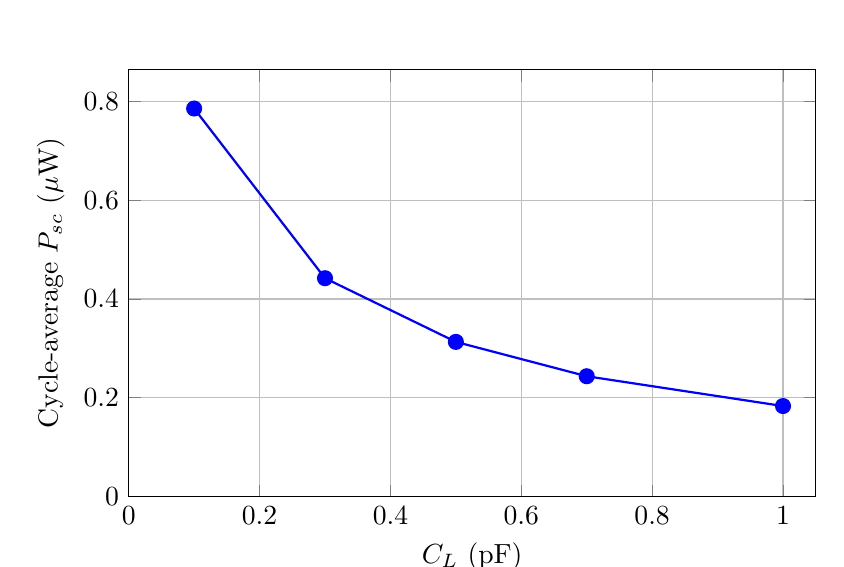
\begin{tikzpicture}\begin{axis}[width=.85\linewidth,height=7cm,xlabel={$C_L$ (pF)},ylabel={Cycle-average $P_{sc}$ ($\mu$W)},grid=major,xmin=0,xmax=1.05,ymin=0,mark size=2.5pt]
\addplot[blue,thick,mark=*] coordinates {(0.1,0.7860142419999999)(0.3,0.442159599)(0.5,0.313113787)(0.7,0.243483722)(1.0,0.18309413900000002)};
\end{axis}\end{tikzpicture}\end{center}
\textbf{Result and mechanism.} Under the stated fixed sizing and 3 ns input slew, $P_{sc}$ decreases monotonically as the load increases. A larger capacitor keeps the output nearer its initial rail during the input overlap interval. For a rising input, the pMOS has a smaller source-drain drop while the output remains high; for a falling input, the nMOS has a smaller drain-source drop while the output remains low. The opposing channel current is reduced in either case. Treating a capacitor as an ordinary resistor and applying a static current divider does not capture this transient feedback.
This trend is conditional on input slew, device sizes, supply, and a fully settling period; it is not a universal claim that total dynamic power falls with load. Here the total supply power actually rises because load switching dominates.
\textbf{Reference corrections.} One supplied DOCX explicitly plots peak short-circuit power because a cycle integral was not obtained; peaks are not average power. The other uses \texttt{AVG} currents and then divides by a period, which is dimensionally incorrect: an average current already has units A. Use either \texttt{INTEG} to obtain charge and divide by T, or a full-period \texttt{AVG} as above. Both references suggest the qualitative decreasing trend, which the corrected simulation confirms under the declared conditions.

\textbf{Reproduce.} Use the command below; optional \texttt{--hspice PATH} selects the installed simulator.
\begin{lstlisting}
python reproduce.py --model D:/cic018.l --work PATH
\end{lstlisting} \texttt{simulate\_and.py} and \texttt{simulate\_power.py} run the questions separately. The \texttt{.sp} subcircuit and both testbenches are provided. Measurement CSVs, voltage checks, waveforms, and conditions are in \texttt{results/and\_gate/} and \texttt{results/power/}. Raw simulator listings stay in the selected work directory. The local process file is never redistributed.
\end{document}
